\documentclass[a4paper, 12pt, twoside]{article}


%------------------------------------------------------------------------
%
% Author                :   Lasercata
% Last modification     :   2022.05.11
%
%------------------------------------------------------------------------


%------ini
\usepackage[utf8]{inputenc}
\usepackage[T1]{fontenc}
\usepackage[french]{babel}
%\usepackage[english]{babel}


%------geometry
\usepackage[textheight=700pt, textwidth=500pt]{geometry}


%------color
\usepackage{xcolor}
\definecolor{ff4500}{HTML}{ff4500}
\definecolor{00f}{HTML}{0000ff}
\definecolor{0ff}{HTML}{00ffff}
\definecolor{656565}{HTML}{656565}

\renewcommand{\emph}{\textcolor{ff4500}}
\renewcommand{\em}{\color{ff4500}}

\newcommand{\strong}[1]{\textcolor{ff4500}{\bf #1}}
\newcommand{\st}{\color{ff4500}\bf}


%------Code highlighting
%---listings
\usepackage{listings}

\definecolor{cbg}{HTML}{272822}
\definecolor{cfg}{HTML}{ececec}
\definecolor{ccomment}{HTML}{686c58}
\definecolor{ckw}{HTML}{f92672}
\definecolor{cstring}{HTML}{e6db72}
\definecolor{cstringlight}{HTML}{98980f}
\definecolor{lightwhite}{HTML}{fafafa}

\lstdefinestyle{DarkCodeStyle}{
    backgroundcolor=\color{cbg},
    commentstyle=\itshape\color{ccomment},
    keywordstyle=\color{ckw},
    numberstyle=\tiny\color{cbg},
    stringstyle=\color{cstring},
    basicstyle=\ttfamily\footnotesize\color{cfg},
    breakatwhitespace=false,
    breaklines=true,
    captionpos=b,
    keepspaces=true,
    numbers=left,
    numbersep=5pt,
    showspaces=false,
    showstringspaces=false,
    showtabs=false,
    tabsize=4,
    xleftmargin=\leftskip
}

\lstdefinestyle{LightCodeStyle}{
    backgroundcolor=\color{lightwhite},
    commentstyle=\itshape\color{ccomment},
    keywordstyle=\color{ckw},
    numberstyle=\tiny\color{cbg},
    stringstyle=\color{cstringlight},
    basicstyle=\ttfamily\footnotesize\color{cbg},
    breakatwhitespace=false,
    breaklines=true,
    captionpos=b,
    keepspaces=true,
    numbers=left,
    numbersep=10pt,
    showspaces=false,
    showstringspaces=false,
    showtabs=false,
    tabsize=4,
    frame=L,
    xleftmargin=\leftskip
}

%\lstset{style=DarkCodeStyle}
\lstset{style=LightCodeStyle}
%Usage : \begin{lstlisting}[language=Caml] ... \end{lstlisting}

%---tcolorbox
\usepackage[many]{tcolorbox}
\DeclareTColorBox{pseudocode}{O{black}O{lightwhite}}{
    breakable,
    outer arc=0pt,
    arc=0pt,
    top=0pt,
    toprule=-.5pt,
    right=0pt,
    rightrule=-.5pt,
    bottom=0pt,
    bottomrule=-.5pt,
    colframe=#1,
    colback=#2,
    enlarge left by=10pt,
    width=\linewidth-\leftskip-10pt,
}


%-------make the table of content clickable
\usepackage{hyperref}
\hypersetup{
    colorlinks,
    citecolor=black,
    filecolor=black,
    linkcolor=black,
    urlcolor=black
}
%Uncomment this and comment above for dark mode
% \hypersetup{
%     colorlinks,
%     citecolor=white,
%     filecolor=white,
%     linkcolor=white,
%     urlcolor=white
% }


%------pictures
\usepackage{graphicx}
%\usepackage{wrapfig}

\usepackage{tikz}
%\usetikzlibrary{babel}             %Uncomment this to use circuitikz
%\usetikzlibrary{shapes.geometric}  % To draw triangles in trees
%\usepackage{circuitikz}            %Electrical circuits drawing


%------tabular
%\usepackage{color}
%\usepackage{colortbl}
%\usepackage{multirow}


%------Physics
%---Packages
%\usepackage[version=4]{mhchem} %$\ce{NO4^2-}$

%---Commands
\newcommand{\link}[2]{\mathrm{#1} \! - \! \mathrm{#2}}
\newcommand{\pt}[1]{\cdot 10^{#1}} % Power of ten
\newcommand{\dt}[2][t]{\dfrac{\mathrm d #2}{\mathrm d #1}} % Derivative


%------math
%---Packages
%\usepackage{textcomp}
%\usepackage{amsmath}
\usepackage{amssymb}
\usepackage{mathtools} % For abs
\usepackage{stmaryrd} %for \llbracket and \rrbracket
\usepackage{mathrsfs} %for \mathscr{x} (different from \mathcal{x})

%---Commands
%-Sets
\newcommand{\N}{\mathbb{N}} %set N
\newcommand{\Z}{\mathbb{Z}} %set Z
\newcommand{\Q}{\mathbb{Q}} %set Q
\newcommand{\R}{\mathbb{R}} %set R
\newcommand{\C}{\mathbb{C}} %set C
\newcommand{\U}{\mathbb{U}} %set U
\newcommand{\seg}[2]{\left[ #1\ ;\ #2 \right]}
\newcommand{\nset}[2]{\left\llbracket #1\ ;\ #2 \right\rrbracket}

%-Exponantial / complexs
\newcommand{\e}{\mathrm{e}}
\newcommand{\cj}[1]{\overline{#1}} %overline for the conjugate.

%-Vectors
\newcommand{\vect}{\overrightarrow}
\newcommand{\veco}[3]{\displaystyle \vect{#1}\binom{#2}{#3}} %vector + coord

%-Limits
\newcommand{\lm}[2][{}]{\lim\limits_{\substack{#2 \\ #1}}} %$\lm{x \to a} f$ or $\lm[x < a]{x \to a} f$
\newcommand{\Lm}[3][{}]{\lm[#1]{#2} \left( #3 \right)} %$\Lm{x \to a}{f}$ or $\Lm[x < a]{x \to a}{f}$
\newcommand{\tendsto}[1]{\xrightarrow[#1]{}}

%-Integral
\newcommand{\dint}[4][x]{\displaystyle \int_{#2}^{#3} #4 \mathrm{d} #1} %$\dint{a}{b}{f(x)}$ or $\dint[t]{a}{b}{f(t)}$

%-left right
\newcommand{\lr}[1]{\left( #1 \right)}
\newcommand{\lrb}[1]{\left[ #1 \right]}
\newcommand{\lrbb}[1]{\left\llbracket #1 \right\rrbracket}
\newcommand{\set}[1]{\left\{ #1 \right\}}
\newcommand{\abs}[1]{\left\lvert #1 \right\rvert}
\newcommand{\ceil}[1]{\left\lceil #1 \right\rceil}
\newcommand{\floor}[1]{\left\lfloor #1 \right\rfloor}
\newcommand{\lrangle}[1]{\left\langle #1 \right\rangle}

%-Others
\newcommand{\para}{\ /\!/\ } %//
\newcommand{\ssi}{\ \Leftrightarrow \ }
\newcommand{\eqsys}[2]{\begin{cases} #1 \\ #2 \end{cases}}

\newcommand{\med}[2]{\mathrm{med} \left[ #1\ ;\ #2 \right]}  %$\med{A}{B} -> med[A ; B]$
\newcommand{\Circ}[2]{\mathscr{C}_{#1, #2}}

\renewcommand{\le}{\leqslant}
\renewcommand{\ge}{\geqslant}

\newcommand{\oboxed}[1]{\textcolor{ff4500}{\boxed{\textcolor{black}{#1}}}} %orange boxed


%------commands
%---to quote french text
\newcommand{\simplecit}[1]{\guillemotleft$\;$#1$\;$\guillemotright}
\newcommand{\cit}[1]{\simplecit{\textcolor{656565}{#1}}}
\newcommand{\quo}[1]{\cit{\it #1}}

%---to indent
\newcommand{\ind}[1][20pt]{\advance\leftskip + #1}
\newcommand{\deind}[1][20pt]{\advance\leftskip - #1}

%---to indent a text
\newcommand{\indented}[2][20pt]{\par \ind[#1] #2 \par \deind[#1]}
\newenvironment{indt}[2][20pt]{#2 \par \ind[#1]}{\par \deind} %Titled indented env

%---title
\newcommand{\thetitle}[2]{\begin{center}\textbf{{\LARGE \underline{\emph{#1} :}} {\Large #2}}\end{center}}


%------Sections
% To change section numbering :
% \renewcommand\thesection{\Roman{section}}
% \renewcommand\thesubsection{\arabic{subsection}}
% \renewcommand\thesubsubsection{\textit \alph{subsubsection}}

% To start numbering from 0
% \setcounter{section}{-1}


%------page style
\usepackage{fancyhdr}
\usepackage{lastpage}

\setlength{\headheight}{18pt}
\setlength{\footskip}{50pt}

\pagestyle{fancy}
\fancyhf{}
\fancyhead[LE, RO]{\textit{\textcolor{black}{\today}}}
\fancyhead[RE, LO]{\large{\textsl{\emph{\texttt{\jobname}}}}}

\fancyfoot[RO, LE]{\textit{\texttt{\textcolor{black}{Page \thepage /}\pageref{LastPage}}}} %Change 'black' to 'white' for dark mode
\fancyfoot[LO, RE]{\includegraphics[scale=0.12]{/home/lasercata/Pictures/1.images_profil/logo/mieux/lasercata_logo_fly_fond_blanc.png}}

% For dark mode :
%/home/lasercata/Pictures/1.images_profil/logo/mieux/lasercata_logo_fly.png


%------init lengths
\setlength{\parindent}{0pt} %To avoid using \noindent everywhere.
\setlength{\parskip}{3pt}


%---------------------------------Begin Document
\begin{document}
    
    %For dark mode :
    % \pagecolor{black}
    % \color{white}
    
    \thetitle{Chapitre 10}{Théorie des graphes}
    
    \tableofcontents
    \newpage
    
    
    \begin{indt}{\section{Introduction}}
        
        \begin{indt}{\subsection{Les origines}}
            \begin{indt}{\subsubsection{Le problème fondateur : les sept ponts de Königsberg}}
                \label{1.1.1}

                \textit{\'Enoncé} : Peut-on effectuer une promenade à Königsberg passant exactement une fois par chacun des ponts ?

                Variante : peut-on le faire en revenant à son point de départ ?

                \begin{center}
                    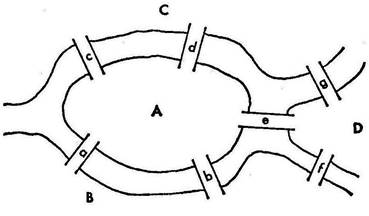
\includegraphics[scale=.5]{pics/pic_1.jpg}
                \end{center}
            \end{indt}

            \vspace{12pt}
            
            \begin{indt}{\subsubsection{Une solution formelle}}
                Présentée par \textsc{Euler} en 1735.

                \begin{indt}{Trois étapes :}
                    (1) Nommage des trois zones et représentation abstraite

                    \begin{center}
                        \begin{tikzpicture}[node distance = 50pt]
                            \node (A) [circle, draw] {A};
                            \node (B) [circle, draw, below right of = A] {B};
                            \node (C) [circle, draw, above right of = A] {C};
                            \node (D) [circle, draw, below right of = C] {D};

                            \draw (A) -- (C) -- (D) -- (B) -- (A);
                            \draw (A) -- (D);

                            \draw (A) to [out=90, in=180] (C);
                            \draw (A) to [out=-90, in=-180] (B);
                        \end{tikzpicture}
                    \end{center}

                    (2) Formalisation de la notion de chemin

                    (3) Démonstration d'impossibilité : il n'existe pas de chemin / circuit eulérien dans ce graphe.
                \end{indt}
            \end{indt}

            \vspace{12pt}
            
            \begin{indt}{\subsubsection{Remarque}}
                Les points (1) et (2) sont les étapes fondatrices de la théorie des graphes vue comme une théorie mathématique.
                Cette théorie a pris une grande ampleur car elle permet de modéliser de nombreux phénomènes.
            \end{indt}
        \end{indt}

        \vspace{12pt}
        
        \begin{indt}{\subsection{De nombreuses applications}}
            \begin{indt}{\subsubsection{Compilation}}
                $\bullet$ Modélisation : on représente le graphe de dépendance entre fichiers.

                \begin{center}
                    \begin{tikzpicture}
                        \node (f) at (0, 0) [rectangle, draw] {
                            \begin{tabular}{l}
                                Foo.ml
                                \\
                                \fbox{open Bar}
                            \end{tabular}
                        };

                        
                        \node (b) at (4, 0) [rectangle, draw] {
                            \begin{tabular}{l}
                                Bar.ml
                                \\
                                \fbox{open Foo}
                            \end{tabular}
                        };

                        \draw[->] (b) to [in=10, out=170] (f);
                        \draw[<-] (b) to [in=-10, out=-170] (f);
                    \end{tikzpicture}
                \end{center}

                $\bullet$ Problème : faisabilité : c'est un problème de détection de cycle.

                Ordre de compilation : choisir un ordre, c'est effectuer un tri topologique du graphe.
            \end{indt}

            \vspace{12pt}
            
            \begin{indt}{\subsubsection{Transports}}
                \label{1.2.2}
                
                $\bullet$ Modélisation : on représente un réseau de transports en commun en représentant les stations liées par les lignes qui y passent.

                $\bullet$ Problème : recherche de chemin le plus court en terme de distance / de temps / nombre de stations.
            \end{indt}

            \vspace{12pt}
            
            \begin{indt}{\subsubsection{Ordonnancement de tâches}}
                $\bullet$ Problème : répartition d'un ensemble de tâches sur un nombre minimal d'unité de calcul.

                $\bullet$ Modélisation : on utilise un graphe d'incompatibilité : on lie les tâches incompatibles entre elles. On veut attribuer une couleur (une unité de calcul) à chaque sommet de sorte qu'aucun sommet ne soit de la même couleur que l'un de ses voisins.
            \end{indt}

            \vspace{12pt}
            
            \begin{indt}{\subsubsection{Construction d'un réseau électrique}}
                \label{1.2.4}
                
                $\bullet$ Problème : on veut raccorder un certain nombre de villes en utilisant le moins de cable possible.

                $\bullet$ Modélisation : on utilise un graphe qui représente les villes liées par des axes annotés par leur longueur. On veut sélectionner des axes pour lier toutes les villes entre elles en utilisant le moins de longueur possible.

                C'est la recherche d'un arbre couvrant de poids minimal.
            \end{indt}
        \end{indt}
        
    \end{indt}

    \vspace{12pt}
    
    \begin{indt}{\section{Bases des graphes}}
        \begin{indt}{\subsection{Vocabulaire}}
            \begin{indt}{\subsubsection{Définition (\textit{graphe})}}
                \begin{indt}{Un graphe est un couple $G = (S, A)$ où :}
                    \label{2.1.1}

                    $\bullet$ $S$ est un ensemble fini de \textit{sommets} ou de \textit{n\oe uds} ;

                    \begin{indt}{$\bullet$ $A$ est un ensemble d'associations entre deux sommets, qui peut prendre plusieurs formes :}
                        $-$ Si $A$ est un ensemble de points de sommets, on dit que $G$ est \textit{non orienté} ;

                        $-$ Si $a = \set{s, s'} \in A$ , on dit que $a$ est une \textit{arête} d'extrémités $s$ et $s'$, que $a$ est \textit{incidente} à $s$ et $s'$, et que $s$ et $s'$ sont \textit{adjacents} ou \textit{voisins} ;

                        $-$ Si $A$ est un ensemble de couples de sommets, on dit que $G$ est \textit{orienté}.
                        \newline
                        Si $a = (s, s') \in A$, on dit que $a$ est un \textit{arc}, que $s'$ est un \textit{successeur} de $s$, que $a$ est un \textit{arc sortant} pour $s$ et \textit{entrant} pour $s'$.
                    \end{indt}
                \end{indt}
            \end{indt}

            \vspace{12pt}
            
            \begin{indt}{\subsubsection{Représentation graphique}}
                On place un point pour chaque sommet et on relie les extrémités d'une même arête (avec une flèche dans le cas orienté).

                Exemple :
                \[
                    G = \lr{\set{A, B, C, D}, \set{\set{A, B}, \set{B, C}, \set{C, A}}}
                \]

                est un graphe non orienté (GNO)

                \begin{center}
                    \begin{tikzpicture}[node distance = 40pt]
                        \node (A) [circle, draw] {A};
                        \node (B) [circle, draw, above right of = A] {B};
                        \node (C) [circle, draw, below right of = A] {C};
                        \node (D) [circle, draw, below right of = B] {D};

                        \draw (A) -- (B) -- (C) -- (A);
                    \end{tikzpicture}
                \end{center}

                Autre exemple :

                \begin{center}
                    \begin{tikzpicture}[node distance = 40pt]
                        \node (A) [circle, draw] {A};
                        \node (B) [circle, draw, right of = A] {B};
                        \node (C) [circle, draw, above of = B] {C};
                        \node (D) [circle, draw, right of = B] {D};

                        \draw[->] (A) to [out=10, in=170] (B);
                        \draw[<-] (A) to [out=-10, in=-170] (B);
                        \draw[->] (D) -- (B);
                        \draw[->] (B) -- (C);
                        \draw[->] (A) to [out=-40, in=-140] (D);
                        \draw[->] (A) -- (C);
                        \draw[->] (C) -- (D);
                    \end{tikzpicture}
                \end{center}

                est la représentation du graphe orienté (GO) :
                \[
                    G = \lr{ \set{A,B,C,D}, \set{(A, B), (B, A), (B, C), (D, B), (A, D), (A, C), (C, D)} }
                \]
                
            \end{indt}

            \vspace{12pt}
            
            \begin{indt}{\subsubsection{Boucles}}
                $\bullet$ Définition (\textit{boucle}) : Une \textit{boucle} dans un graphe est une arête / un arc dont les extrémités sont égales.

                $\bullet$ Remarque : la définition \ref{2.1.1} (page \pageref{2.1.1}) empêche la présence de boucles dans les GNO.
                On peut les autoriser en considérant non pas des paires de sommets, mais des \textit{multi-ensembles} de cardinal 2.

                On pourrait aussi utiliser les \textit{multi-ensembles} pour autoriser les multi-arêtes (plusieurs arêtes entre 2 sommets donnés, comme ent \ref{1.1.1}, page \pageref{1.1.1}, mais c'est H.P : $A$ sera toujours un ensemble).
            \end{indt}

            \vspace{12pt}
            
            \begin{indt}{\subsubsection{Degré}}
                $\bullet$ Définition (\textit{degré}) : Soit $G = (S, A)$ un GNO et $s \in S$.

                Le degré de $s$, noté $d(s)$  est le nombre de voisins de $s$ :
                \[
                    d(s) = \abs{\vphantom{\dfrac a a}\!\set{a \in A\ |\ s \in a}}
                \]
                
                $\bullet$ Définition (\textit{degré entrant / sortant}) : Soit $G = (S, A)$ un GO et $s \in S$.

                Le \textit{degré entrant} (resp. \textit{sortant}) de $s$, noté $d_-(s)$  (resp. $d_+(s)$), est le nombre d'arcs entrants (resp. sortant) pour $s$ :
                \[
                    d_-(s) = \abs{\vphantom{\dfrac a a}\!\set{a \in A\ |\ \exists s' \in S\ |\ a = (s', s)}}
                \]
                \[
                    d_+(s) = \abs{\vphantom{\dfrac a a}\!\set{a \in A\ |\ \exists s' \in S\ |\ a = (s, s')}}
                \]
                
                \begin{indt}{$\bullet$ Proposition (formule de la somme des degrés) : Soit $G = (S, A)$ un graphe.}
                    (1) Si $G$ est un GNO sans boucle,
                    \[
                        \sum_{s \in S} d(s) = 2\abs{A}
                    \]

                    (2) Si $G$ est un GO,
                    \[
                        \sum_{s \in S} d_-(s) = \sum_{s \in S} d_+(s) = \abs{A}
                    \]
                \end{indt}

                \begin{indt}{$\square$ Démonstration :}
                    (1) On compte les extrémités d'arêtes :

                    $-$ Une arête compte pour deux extrémités car ce n'est pas une boucle, donc il y en a $2\abs A$ ;

                    $-$ $\forall s \in S$, $s$ est extrémité de $d(s)$ arêtes, donc il y en a
                    \[
                        \sum_{s \in S} d(s)
                    \]
                    
                    (2) Par récurrence sur $\abs A$ :

                    $-$ Si $\abs A = 0,\ \forall s \in S,\ d_+(s) = d_-(s) = 0$ Ok.

                    $-$ Héréditée : si $\abs A > 0$, alors $\exists (s, s') \in A$.

                    On note $G' = (S,\ a \setminus \set{(s, s')})$.

                    Par hypothèse de récurrence :
                    \[
                        \abs A - 1 = \abs{A \setminus \set{(s, s')}} = \sum_{v \in S \setminus \set{s'}} d_-(v) + \underbrace{d_-(s) - 1}_{\text{degré sortant de $s$ dans $G$}}
                    \]
                    
                    Donc $\abs A = \displaystyle \sum_{v \in S} d_-(v)$

                    De même pour les degrés entrants, en considérant $s'$ plutôt que $s$
                    $\blacksquare$
                \end{indt}

                \vspace{6pt}
                
                $\bullet$ Corollaire (\textit{handshaking lemma}) : Tout GNO sans boucle possède un nombre pair de sommets de degré impair.

                \begin{indt}{$\square$ Démonstration :}
                    \[
                        2\N \ni 2\abs A
                        = \sum_{s \in S} d(s)
                        = \underbrace{\sum_{\substack{s \in S \\ d(s) \in 2\N}} d(s)}_{\in 2\N} + \underbrace{\sum_{\substack{s \in S \\ d(s) \in 2\N + 1}} d(s)}_{\substack{\text{de la parité du nombre} \\ \text{de sommets de degré impair}}}
                    \]
                    $\blacksquare$
                \end{indt}
                
                \vspace{12pt}

                Contre-exemple en cas de boucle :

                \begin{center}
                    \begin{tikzpicture}
                        \node (A) [circle, draw] {A};
                        \draw (A) to [in=90, out=0, looseness=5] (A);
                    \end{tikzpicture}
                \end{center}
            \end{indt}

            \vspace{12pt}
            
            \begin{indt}{\subsubsection{Graphes étiquetés}}
                $\bullet$ Définition (\textit{graphe étiqueté}) : Soit $G = (S, A)$ un graphe.

                On dit que $G$ est :

                $-$ \textit{étiqueté} s'il est muni d'une fonction $f : A \longrightarrow V$ où $V$ est un ensemble de valeurs appelées les \textit{étiquettes}.

                $-$ \textit{pondéré} s'il est étiquetté par des nombres (entiers / réels) : on parle de \textit{poids} plutôt que d'étiquette.

                Exemple : \ref{1.2.2} (page \pageref{1.2.2}), \ref{1.2.4} (page \pageref{1.2.4}),

                \begin{center}
                    \begin{tikzpicture}[node distance = 60pt]
                        \node (A) at (0, 0) [circle, draw] {A};
                        \node (B) [circle, draw, above right of = A] {B};
                        \node (C) [circle, draw, below right of = A] {C};
                        \node (D) [circle, draw, below right of = B] {D};
                        
                        \draw[->] (A) to [out=90, in=180] node [above left] {5} (B);
                        \draw[->] (B) to [out=-90, in=0] node [above left] {10} (A);
                        
                        \draw[->] (D) to [out=90, in=0] node [above right] {5} (B);
                        
                        \draw[->] (B) to [out=-70, in=70] node [left] {3} (C);
                        
                        \draw[->] (A) to [out=-90, in=180] node [above right] {3} (C);
                        
                        \draw[->] (C) to [out=0, in=-90] node [above left] {5} (D);
                        
                        \draw[->] (A) to [out=-135, in=-45, looseness=3] node [below] {-4} (D);
                    \end{tikzpicture}
                \end{center}

                %En MPI : les automates finis.
            \end{indt}

            \vspace{12pt}
            
            \begin{indt}{\subsubsection{Graphes bipartis}}
                $\bullet$ Définition (\textit{graphes bipartis}) : Soit $G = (S, A)$ un graphe.

                On dit que $G$ est \textit{biparti} s'il existe une partition de $S$ $(U, V)$ telle que pour toute arête $a$, une extrémité de $a$ appartienne à $U$ et l'autre à $V$.

                Exemple ($\textcolor{red}{U}, V$) :
                \begin{center}
                    \begin{tikzpicture}
                        \foreach \k in {1, 3, 5} {
                            \node (\k) at (\k, 0) [circle, fill] {};
                        }
                        
                        \foreach \k in {2, 4, 6} {
                            \node (\k) at (\k, 0) [circle, draw, color=red] {};
                        }

                        \node (7) [above of = 2, circle, fill] {};
                        \node (8) [above of = 5, circle, draw, color=red] {};
                        
                        \draw (1) -- (2) -- (3) -- (4) -- (5) -- (6);
                        \draw (2) -- (7);
                        \draw (5) -- (8);
                        
%                         \foreach \i/\j in {2/0, 4/0, 5/1, 6/0} {
%                             \draw [color=red] (\i, \j) circle (.3);
%                         }
                    \end{tikzpicture}
                \end{center}
                
                Peut aussi se représenter :
                
                \begin{center}
                    \begin{tikzpicture}                        
                        \foreach \k/\i/\j in {2/0/0, 4/0/-2, 6/0/-3, 8/0/-4} {
                            \node (\k) at (\i, \j) [circle, draw, color=red] {};
                        }
                        
                        \foreach \k/\i/\j in {1/2/0, 7/2/-1, 3/2/-2, 5/2/-3} {
                            \node (\k) at (\i, \j) [circle, fill] {};
                        }
                        
                        \draw (1) -- (2) -- (3) -- (4) -- (5) -- (6);
                        \draw (2) -- (7);
                        \draw (5) -- (8);
                    \end{tikzpicture}
                \end{center}
                
                Remarque : un graphe biparti est $2$-colorable.
            \end{indt}
        \end{indt}
    \end{indt}
    
    
    
\end{document}
%--------------------------------------------End
